\documentclass[1p]{elsarticle}

\usepackage{amsmath}
\usepackage{amssymb}
\usepackage{graphicx}
\usepackage{subfigure}
\usepackage[colorlinks,unicode,linkcolor=black]{hyperref}
\usepackage{listings}
\lstset{
    language=C++,
    basicstyle=\small,
    columns=flexible,
    showstringspaces=false,
    numbers=left,
    numberstyle=\tiny,
    frame=leftline
    }
\newcommand{\code}[1]{\lstinline|#1|}
\newcommand{\figref}[1]{Fig.~\ref{#1}}

%
% mathematical commands
%
\newcommand {\re} {\text{Re}}
\newcommand {\im} {\text{Im}}
\newcommand {\de} {\mbox{d}}
\newcommand {\ii} {\text{i}}
\newcommand {\ee} {\text{e}}
\newcommand {\mathbi}[1] {\textbf{\em #1}}
\newcommand {\sign} {\text{sign}}
\newcommand {\bra}[1] {\langle #1 \mid}
\newcommand {\ket}[1] {\mid #1 \rangle}
\newcommand {\braket}[2] {\langle #1 \mid #2 \rangle}
\newcommand {\mean}[1] {\langle #1 \rangle}
\newcommand {\sech} {\text{sech}}
\newcommand {\conj} {\ast}

\newcommand {\rem}[1]{}


\journal{Journal of Parallel and Distributed Computing}

\begin{document}

\begin{frontmatter}

\title{Programming OpenCL and CUDA:\\a Case Study Using Modern C++ Libraries}

\author{Karsten Ahnert}
\ead{karsten.ahnert@gmx.de}
\address{
Institut f\"ur Physik und Astronomie, Universit\"at Potsdam,\\
Karl-Liebknecht-Strasse 24/25, 14476 Potsdam-Golm, Germany
}

\author{Denis Demidov}
\ead{ddemidov@ksu.ru}
\address{
Kazan Branch of Joint Supercomputer Center,
Russian Academy of Sciences,\\
Lobachevsky st. 2/31, 420008 Kazan, Russia
}

\author{Karl Rupp}
\ead{rupp@iue.tuwien.ac.at}
\address{Mathematics and Computer Science Division,
Argonne National Laboratory \\
9700 South Cass Avenue, Argonne, IL 60439, USA
}

\begin{abstract}
    We present a comparison of several modern C++ libraries intended for OpenCL
    and CUDA programming. The comparison is based on odeint, a framework for
    the solution of ordinary differential equations. Odeint is designed in a
    very flexible way such that the algorithms are completely independent from
    the underlying containers and even from the basic algebraic computations.
    This allows to effectively use libraries such as VexCL, ViennaCL, or Thrust
    to solve ODEs with either OpenCL or CUDA technologies. We found that OpenCL
    and CUDA work equally well for problems of large sizes, while OpenCL has
    higher overhead for smaller problems.
    % [KR]: The abstract should end with a more catchy phrase

    % [DD]: Perhaps we should say something to the effect of: since CUDA and
    % OpenCL performance seems to be on par, we beleive that main factor for
    % the library to work with should be convenience of its interface and
    % availability of required functions. In the context of our work (ODE
    % solving) OpenCL libraries proved to be more convenient due to
    % availability of expression templates.
\end{abstract}

\begin{keyword}
    GPGPU \sep OpenCL \sep CUDA \sep Modern C++ libraries \sep odeint \sep
    VexCL \sep ViennaCL \sep Thrust
\end{keyword}

\end{frontmatter}





%
% INTRODUCTION
%
\section{Introduction}

Recently, general purpose computing on graphics processing units (GPGPU) has
acquired considerable momentum in the scientific community. This is confirmed
both by increasing numbers of GPGPU-related publications and GPU based
supercomputers in the Top
500\footnote{\href{http://top500.org/}{http://top500.org/}} list. Major
programming frameworks are NVIDIA CUDA and OpenCL.  The former is a proprietary
parallel computing architecture developed by NVIDIA for general purpose
computing on NVIDIA graphics adapters, and the latter is an open, royalty-free
standard for cross-platform, parallel programming of modern processors
maintained by the Khronos group. By nature, the two frameworks have their
distinctive pros and cons. CUDA has a more mature programming environment with
larger set of scientific libraries; but it is only supported on NVIDIA
hardware. OpenCL is supported on wide range of hardware, but its native API
requires much larger amount of boilerplate code from a developer.

Both technologies are able to provide scientists with the vast computational
resources of modern GPU cards at the price of a steep learning curve.
Programmers need to familiarize
themselves with a new programming language and, more importantly, with a
new programming paradigm. However, the entry price may be lowered with help of
specialized libraries. The CUDA Toolkit includes several such libraries (BLAS
implementation, Fast Fourier Transform, Thrust and others). OpenCL lacks
standard libraries, but there are a number of third-party projects aimed at
developing both CUDA and OpenCL programs.

This paper presents comparison of several modern C++ libraries aimed at ease of
GPGPU development. We look at both convenience and performance of the libraries
under consideration in the context of solving ordinary differential equations.
The comparison is based on odeint, modern C++ library for solution of ODEs.
The GPGPU libraries considered in this work are Thrust, VexCL, and ViennaCL:

% [KR]: We need to define the scope of this work. We are investigating ODEs
% only, which we have to clarify.  There is a lot of GPGPU for dense linear
% algebra, sparse solvers, and molecular dynamics approaches. We don't consider
% any of these.

% [DD]: Is `the context of solving ordinary differential equations` not enough
% for this purpose? Or should we explicitly state that we are not intersted in
% the topics you mentioned?

\begin{description}
    \item[Odeint] is a modern C++
        library\footnote{\href{http://odeint.com}{http://odeint.com}} for
        numerically solving Ordinary Differential Equations \cite{OdeintRef1,
        OdeintRef2}. It is developed in a generic way using Template
        Metaprogramming which leads to extraordinary high flexibility at top
        performance. The numerical algorithms are implemented independently of
        the underlying arithmetics.  This results in a broad
        applicability of the library, especially in non-standard environments.
        For example, odeint supports matrix types, arbitrary precision
        arithmetics and can be easily adopted to use either CUDA or OpenCL
        frameworks.  Odeint is used in this work as a framework for comparison
        of other libraries.
    \item[Thrust] is a parallel algorithms
        library\footnote{\href{http://thrust.github.com}{http://thrust.github.com}}
        which resembles the C++ Standard Template Library \cite{ThrustRef}.
        Thrust's high-level interface greatly enhances developer productivity
        while enabling performance portability between GPUs and multicore CPUs.
        Thrust is distributed with NVIDIA CUDA Toolkit since version 4.1.
    \item[VexCL] is vector expression template
        library\footnote{\href{https://github.com/ddemidov/vexcl}{https://github.com/ddemidov/vexcl}}
        for OpenCL \cite{VexCLRef}. It has been created for ease of OpenCL
        development with C++.  VexCL strives to reduce the amount of boilerplate
        code needed to develop OpenCL applications. The library provides a
        convenient and intuitive notation for vector arithmetic, reduction, and
        sparse matrix-vector multiplication.  Multi-device and even
        multi-platform computations are supported. 
    \item[ViennaCL] (The Vienna Computing Library) is a scientific computing
        library\footnote{\href{http://viennacl.sourceforge.net}{http://viennacl.sourceforge.net}}
        written in C++ and based on OpenCL \cite{ViennaCLRef}. It allows
        simple, high-level access to the vast computing resources available on
        parallel architectures such as GPUs and is primarily focused on common
        linear algebra operations (BLAS levels 1, 2 and 3) and the solution of
        large systems of equations by means of iterative methods with optional
        preconditioner.
\end{description}

CUDA and OpenCL differ in their handling of compute kernels compilation. In
CUDA the compute kernels are compiled to PTX code together with the host
program. The PTX is pseudo-assembler language which is compiled at runtime for
the specific NVIDIA device it is being run on. Since PTX is already very
low-level, this just-in-time kernel compilation has low overhead. In OpenCL the
compute kernels are compiled at runtime from high level sources. This adds an
overhead which is particularly noticeable for smaller sized problems. The
pre-compilation to some low-level pseudo-code is not feasible in OpenCL because
it has to support wide range of hardware.

The approach to generation and compilation of the compute kernels is one of the
main differences between the OpenCL libraries we considered.  ViennaCL has
limited set of predefined kernels, which functionally coincides with BLAS level
1 routines.  These kernels are compiled in batch at the program start to allow
for faster initialization. However, due to this design decision each vector
expression may result in launch of more than one kernel.  On the other hand,
VexCL generates and compiles an OpenCL program with a single kernel for each
vector expression it encounters.  This leads to potentially higher
initialization overhead, but should prove to be more effective in the long
runs. It should be noted that main aim of ViennaCL is provision of iterative
solvers for large sparse systems of equations. In this context complex vector
expressions are rare and we believe that authors of ViennaCL made correct
design decision.  However, we think it is interesting to compare approaches of
VexCL and ViennaCL.

% [DD]: what do you think of: The other difference between CUDA and OpenCL is
% that CUDA supports subset of C++ language in compute kernels, while OpenCL
% kernels are written in subset of C99. Therefore, CUDA programmers may use
% template metaprogramming techniques which may lead to more efficient and
% compact code.  Native OpenCL API does not provide this ability, but modern
% C++ libraries such as those considered in this work...





%
% ADAPTING ODEINT
%
\section{Adapting odeint}

Odeint provides a mechanism which lets the user change the way 
elementary numerical computations are performed. This mechanism consists of a
combination of state type, algebra and operations. The state type represents the
state of the ODE being solved and is usually a vector type like
\code{std::vector<>} or \code{std::array<>}. The algebra is responsible for
iterating through all elements of the state whereas the operations are
responsible for the elementary operations. An example of using a range algebra
is provided below:
\begin{lstlisting}
typedef std::array<double, 3> state_type;
state_type x1, x2;
// Initialize x1 and x2.

double dt = 0.1;
odeint::range_algebra algebra;
// The following line computes x1 = dt * x2 for all elements of x1 and x2:
algebra.for_each2(x1, x2, default_operations::scale_sum1(dt));
\end{lstlisting}
Here \code{for_each2} is used, which means that
two state types are iterated. The operation is a \code{scale_sum1} which simply
calculates \code{x1[i] = dt * x2[i]}. Odeint provides a set of predefined
algebras, which includes:
\begin{itemize}
    \item \code{range_algebra}: default algebra which works on Boost.Ranges
    \item \code{array_algebra}: specialized algebra for boost::array
    \item \code{fusion_algebra}: algebra for compile-time sequences like
        \code{boost::fusion::vector}, \code{std::tuple}, etc.
    \item \code{vector_space_algebra}: algebra for vector space types which
        provide overloaded arithmetic operators for elementwise operations.
\end{itemize}

% [KR]: A few more details would be nice in the previous paragraph...

Many libraries for vector and matrix types provide expression templates for the
elementary operations. Such libraries do not need an own algebra but can be
used with the \code{vector_space_algebra} and the \code{default_operations}
which simply calls the operations directly on the matrix or vector type. In
this case only odeint resizing mechanism has to be adapted.

In the following subsections we describe odeint adaptation for GPGPU libraries
under consideration. We should mention that odeint now supports all of the
mentioned libraries natively. However, providing adaptation examples serves our
goal of comparing ease of use of the libraries.

\subsection{Thrust}
\subsection{VexCL}
\subsection{ViennaCL}














\section{Numerical experiments}

Ordinary differential equations play a major role in many scientific
disciplines. They occur naturally in the context of mechanical
systems, like granular and molecular dynamics~--- in fact the Newtonian
and Hamiltonian mechanics are formulated as ordinary differential
equations. Many other applications can be found in such diverse
fields, like biology and neuroscience, chemistry, social sciences, in
nonlinear science. Furthermore, ODEs are used to solve partial
differential equations (PDEs) numerically, they occur by discretization of
the spatial coordinates.

Odeint usually solves the initial value problem (IVP) of ordinary differential
equations.
\begin{equation}
\frac{\de x}{\de t } = \dot{x} = f(x , t) \quad \text{,} \quad \quad x(0) =
x_0.
\end{equation}
Here, $x$ is the dependent variable. It is usually a vector of real
number but also complex numbers are allowed. $t$ is the independent
variable. We will call it time throughout the article and we will
denote the time derivative with $\de x / \de t = \dot{x}$. $f(x,t)$
is the system function and defines the ODE.

Numerous methods on solving ODEs exist \cite{HairerSolvingODEI,
HairerSolvingODEII, HairerGeometricNumericalIntegration2006}. They are usually
categorized in the field of numerical analysis. Odeint implements the most
prominent of these methods, for example the classical Runge-Kutta-Methods and
Runge-Kutta-Fehlberg methods, multistep methods (Adams-Bashforth-Moulton),
symplectic Runge-Kutta-Nystr\"om methods, and implicit methods (Rosenbrock and
implicit Euler).

Typical use cases for solving ODEs on GPUs are large systems of
coupled ODEs which occur as discretizations of PDEs, or lattice
ODEs. Another use case are parameter studies, where one wants to study
the dependence of an ODE on some parameters. Here, one creates one
large ODE which consists of many small uncoupled ODEs, each with a
different parameter set. This one large system is then solved at once,
hence all small ODEs are solved simultaneously.




%
% DAMPED OSCILLATOR
%
\subsection{Damped Harmonic Oscillator Ensemble}

The first example is a set of damped driven oscillators 
\begin{equation} \label{eq:dampedsystem}
    \dot{x} = \omega y + \varepsilon x \quad \text{,} \quad \quad
    \dot{y} = -\omega x + \varepsilon y
\end{equation}
with $\varepsilon = \varepsilon_0 + \varepsilon_a \cos \left( \omega_d
t \right)$. $\omega$ is the natural frequency of the oscillator and
$\varepsilon$ is the time dependent damping constant.  Note, that this form is
not the classical form of a damped oscillator, but can be derived easily from
$\ii \dot{\Psi} = \omega \Psi + \ii \varepsilon \Psi$ with $\Psi = x + \ii y$.


The Thrust version of the system functor for the damped harmonic oscillator
ensemble example is presented below. The functor holds model parameters and
provides \code{operator()} with a signature required by the odeint library. The
state type is represented by \code{thrust::device_vector<double>}:
\begin{lstlisting}
typedef thrust::device_vector<double> state_type;

struct oscillator {
    size_t N;
    double omega, amp, offset, omega_d;

    oscillator(size_t N, double omega, double amp, double offset, double omega_d)
        : N(N), omega(omega), amp(amp), offset(offset), omega_d(omega_d) { }

    void operator()(const state_type &x, state_type &dxdt, double t) const;
};
\end{lstlisting}
$X$ and $Y$ components of the state are held in first and second halves of the
vector correspondingly.  \code{operator()} packs the state components into a
zip iterator and passes them to \code{thrust::for_each} algorithm together with
the provided device functor:
\begin{lstlisting}[firstnumber=12]
struct oscillator_functor;

void oscillator::operator()(const state_type &x, state_type &dxdt, double t) const {
    double eps = offset + amp * cos(omega_d * t);
    thrust::for_each(
        thrust::make_zip_iterator(
            thrust::make_tuple(
                boost::begin(x), boost::begin(x) + N,
                boost::begin(dxdt), boost::begin(dxdt) + N ) ),
        thrust::make_zip_iterator(
            thrust::make_tuple(
                boost::begin(x) + N, boost::end(x),
                boost::begin(dxdt) + N, boost::end(dxdt) ) ),
        oscillator_functor(omega, eps) );
}
\end{lstlisting}
The device functor unpacks individual components and applies the required
operations to the derivative part:
\begin{lstlisting}[firstnumber=last]
struct oscillator_functor {
    double eps, omega;

    oscillator_functor(double omega, double eps) : omega(omega), eps(eps) {}

    template< class T >
    __host__ __device__ void operator()(T t) const {
        double x = thrust::get< 0 >( t );
        double y = thrust::get< 1 >( t );
        thrust::get<2>(t) = eps * x + omega * y;
        thrust::get<3>(t) = eps * y - omega * x;
    }
};
\end{lstlisting}
This technique allows for the computation of the system function in single
efficient pass resulting in a single CUDA kernel launch.


The system functor for the VexCL version of the damped harmonic oscillator
example is much simpler than the Thrust variant because VexCL supports a rich
set of vector expressions. The state is represented by the
\code{vex::multivector<double,2>} type which holds two instances of
\code{vex::vector<double>} and transparently dispatches all operations to the
underlying components. The code for \code{operator()} body practically
coincides with the problem statement \eqref{eq:dampedsystem}: 
\begin{lstlisting}
typedef vex::vector<double> vector_type;
typedef vex::multivector<double, 2> state_type;

struct oscillator {
    double omega, amp, offset, omega_d;

    oscillator(double omega, double amp, double offset, double omega_d)
        : omega(omega), amp(amp), offset(offset), omega_d(omega_d) { }

    void operator()(const state_type &x, state_type &dxdt, double t) const {
        double eps = offset + amp * cos(omega_d * t);
        dxdt(0) = eps * x(0) + omega * x(1);
        dxdt(1) = eps * x(1) - omega * x(0);
    }
};
\end{lstlisting}


The drawback of this variant is that it leads
to two kernel launches (one per each vector assignment) and results in
suboptimal performance. We are not able to use simple multivector arithmetic
operations here because components in the right hand sides of the assignments
are interchanged.  Fortunately, VexCL provides notation for such
multi-operations.  Assignment of a tuple of expressions to a multivector leads
to generation and launch of single efficient OpenCL kernel. This notation is
only slightly more cumbersome than the above variant:
\begin{lstlisting}[firstnumber=11]
double eps = offset + amp * cos(omega_d * t);
dxdt = std::make_tuple(     eps * x(0) + omega * x(1),
                            eps * x(1) - omega * x(0)   );
\end{lstlisting}

The ViennaCL version of the damped harmonic oscillator example uses
\code{boost::fusion::vector} to pack coordinate components of the state into a
single type. Individual components are instances of
\code{viennacl::vector<double>} type.

ViennaCL, as well as VexCL, supports expression templates for a limited set of
vector operations (closely corresponding to Level 1 BLAS routines). More
complex expressions may be built with help of the ViennaCL kernel generator
interface, which supports single- or multiple-operations kernels. The required
notation is a bit more cumbersome than that of VexCL library. OpenCL kernels
here are generated from symbolic expressions involving explicit symbolic types:
\begin{lstlisting}
typedef viennacl::vector<double> vector_type;
typedef fusion::vector<vector_type, vector_type> state_type;

struct oscillator {
    double omega, amp, offset, omega_d;

    viennacl::generator::symbolic_vector<0, double> sym_dx;
    viennacl::generator::symbolic_vector<1, double> sym_dy;
    viennacl::generator::symbolic_vector<2, double> sym_x;
    viennacl::generator::symbolic_vector<3, double> sym_y;
    viennacl::generator::cpu_symbolic_scalar<4, double> sym_eps;
    viennacl::generator::cpu_symbolic_scalar<5, double> sym_omega;
    viennacl::generator::custom_operation op;

    oscillator(double omega, double amp, double offset, double omega_d)
        : omega(omega), amp(amp), offset(offset), omega_d(omega_d),
          op(sym_dx = sym_eps * sym_x + sym_omega * sym_y,
             sym_dy = sym_eps * sym_y - sym_omega * sym_x,
             "oscillator")
    { }

    void operator()( const state_type &x, state_type &dxdt, double t );
};
\end{lstlisting}

This requires more of boilerplate code but the resulting expression tree
carries information of whether two terminals represent the same vector
instance. This in principle allows generation of more effective code. The
\code{operator()} unpacks \code{boost::fusion::vector} container and launches
the generated kernel:
\begin{lstlisting}[firstnumber=24]
void oscillator::operator()( const state_type &x, state_type &dxdt, double t ) {
    vector_type &X  = const_cast<vector_type&>( fusion::at_c<0>(x) );
    vector_type &Y  = const_cast<vector_type&>( fusion::at_c<1>(x) );
    vector_type &dX = fusion::at_c<0>(dxdt);
    vector_type &dY = fusion::at_c<1>(dxdt);

    double eps = offset + amp * cos(omega_d * t);
    viennacl::ocl::enqueue( op(dX, dY, X, Y, eps, omega) );
}
\end{lstlisting}




%
% PHASE OSCILLATORS
%
\subsection{Chain of Coupled Phase Oscillators}

As a second example we consider a chain of coupled phase oscillators. A
phase oscillator describes the dynamics of an autonomous oscillator
\cite{Synchronization-Pikovsky,Kuramoto-84}. Its evolution is
governed by the phase, a $2\pi$ periodic variable which grows linearly
in time $\de \phi / \de t = \omega$. $\omega$ is here the phase
velocity. Due to the absence of any information about the amplitude of
the oscillator, interesting behaviour can only be observed if many of
such oscillators are coupled. In fact, such a system can be used to study
such divergent phenomena like synchronization, wave and pattern
formation, phase chaos, or oscillation death \cite{}. It is a
prominent example of an emergent system where the coupled system shows
more complex behaviour than its constitutes.

The concrete example we analyze here is a chain of nearest-neighbor
coupled phase oscillators:
\begin{equation} \label{eq:phasesystem}
    \dot{\phi}_i = \omega_i + \sin( \phi_{i+1} - \phi_i) + \sin( \phi_i
    - \phi_{i-1}).
\end{equation}
The index $i$ denotes here the $i$-th phase in the chain. Note, that
the phase velocity might be heterogeneous.

The Thrust version for the coupled phase oscillator chain looks very similar to
the damped oscillator example. Again, we use a zip iterator to pack required
components and process the resulting sequence with single sweep of the
\code{for_each} algorithm. The only difference here is that we need values of
neighboring vector elements. In order to provide the values, we use Thrust's
permutation iterator, so that \code{operator()} of the system functor looks
like
\begin{lstlisting}
thrust::for_each(
    thrust::make_zip_iterator(
        thrust::make_tuple(
            x.begin(),
            thrust::make_permutation_iterator( x.begin(), prev.begin() ),
            thrust::make_permutation_iterator( x.begin(), next.begin() ),
            omega.begin(),
            dxdt.begin() ) ),
    thrust::make_zip_iterator(
        thrust::make_tuple(
            x.end(),
            thrust::make_permutation_iterator( x.begin(), prev.end() ),
            thrust::make_permutation_iterator( x.begin(), next.end() ),
            omega.end(),
            dxdt.end() ) ),
    sys_functor()
    );
\end{lstlisting}
\code{prev} and \code{next} are instances of
\code{thrust::device_vector<size_t>} holding indices to left and right vector
elements and initialized as
\begin{lstlisting}
thrust::counting_iterator<size_t> c(0);
thrust::copy(c, c + N - 1, prev.begin() + 1);
prev[0] = 0;     // prev = { 0, 0, 1, 2, 3, ..., N-1 }
thrust::copy(c + 1, c + N, next.begin());
next[N-1] = N-1; // next = { 1, 2, 3, ..., N-1, N-1 }
\end{lstlisting}

The VexCL version of the example is presented below.  Again, it is the most
concise variant since VexCL provides native support for the user-defined
stencils operations. The sum of sines in \eqref{eq:phasesystem} is encoded
using the \code{vex::StencilOperator<>} class template.  Template parameters
are the body string for the generated OpenCL function encoding required
operation, width and center point of the stencil, and its return type. Once the
stencil operator is defined, the functor's \code{operator()} is implemented
with a single line of code:
\begin{lstlisting}
typedef vex::vector<double> state_type;
extern const char oscillator_body[] = "return sin(X[-1] - X[0]) + sin(X[0] - X[1]);";

struct phase_oscillators {
    const state_type &omega;
    vex::StencilOperator< double, 3, 1, oscillator_body > S;
    phase_oscillators(const state_type &omega) : omega(omega), S(omega.queue_list()) { }
    void operator()(const state_type &x, state_type &dxdt, double t) const {
        dxdt = omega + S(x);
    }
};
\end{lstlisting}


Unfortunately, ViennaCL does not provide stencil operations required for
the problem at hand, so we had to fallback to hand-coded OpenCL kernel:
\begin{lstlisting}
static const char phase_oscillator_source[] =
    "#pragma OPENCL EXTENSION cl_khr_fp64: enable\n"
    "kernel void oscillator(\n"
    "        uint n,\n"
    "        global double *dx,\n"
    "        global const double *x,\n"
    "        global const double *omega\n"
    "        )\n"
    "{\n"
    "    for(uint i = get_global_id(0); i < n; i += get_global_size(0)) {\n"
    "        double X0 = x[i];\n"
    "        double Xl = i > 0 ? x[i - 1] : X0;\n"
    "        double Xr = i + 1 < n ? x[i + 1] : X0;\n"
    "        dx[i] = omega[i] + sin(Xl - X0) + sin(X0 - Xr);\n"
    "    }\n"
    "}\n";
\end{lstlisting}
ViennaCL provide convenient mechanism for compilation and launching of custom
kernels, so this was a pleasant experience in comparison with native OpenCL
API. This low-level variant expectedly turned out to be the most effective one
(see the Results section):
\begin{lstlisting}[firstnumber=last]
typedef viennacl::vector<double> state_type;

struct phase_oscillators {
    const state_type &omega;

    sys_func(const state_type &omega) : omega(omega) {
        viennacl::ocl::current_context().add_program(phase_oscillator_source,
            "oscillator_program").add_kernel("oscillator");
    }

    void operator()(const state_type &x, state_type &dxdt, double t) const {
        viennacl::ocl::kernel &step = viennacl::ocl::current_context().get_program(
            "oscillator_program").get_kernel("oscillator");

        viennacl::ocl::enqueue( step(static_cast<cl_uint>(x.size()), dxdt, x, omega) );
    }
};
\end{lstlisting}








%
% DISORDERED LATTICES
%
\subsection{Disordered Hamiltonian Lattice}

\rem{
Another example for our performance and usage study is a strongly
nonlinear disordered Hamiltonian lattice. Its equations of motion are
governed by
\begin{equation}
\frac{\de q_{i,j}}{\de t} = p_{i,j} \quad \text{,} \quad \quad \frac{\de
p_{i,j}}{\de t} = - \omega_{i,j}^2 q_i - \beta q_{i,j}^3 + \Delta_d q_{i,j}
\,\,\text{.}
\label{eq:disordered_ham}
\end{equation}
Here, $\Delta_d q_{i,j}$ denotes the two-dimensional discreet Laplacian
$\Delta_d
q_{i,j}=q_{i+1,j}+q_{i-1,j}+q_{i,j+1}+q_{i,j-1}-4q_{i,j}$. Such
systems are widely used in theoretical physics to study phenomena
like Anderson localization or thermalization.

An important property of \eqref{eq:disordered_ham} is its Hamiltonian
nature. It can be obtained from a Hamiltonian and the energy and phase
volume is conserved during its evolution. To account for these
properties, a special class of solvers exists, namely symplectic
solvers. Odeint implements three different variants of such solvers,
all are of the Runge-Kutta-Nystrom type.
}

\begin{equation} \label{eq:latticesystem}
    \frac{dp}{dt} = -\Delta Kq + Dq - \beta q^3.
\end{equation}

The natural choice for the implementation of \eqref{eq:latticesystem} is a
sparse matrix-vector product. Unfortunately, Thrust provides neither a sparse
matrix type, nor sparse matrix-vector product operation.  We had to combine
Thrust with the CUSPARSE library in order to implement this example. CUSPARSE
contains a set of basic linear algebra subroutines used for handling sparse
matrices and is included in CUDA Toolkit distribution as well as Thrust
library. Another possibility would be to use an open source Cusp library~--- a
library for sparse linear algebra and graph computations on CUDA
\cite{CuspRef}. 

All of the libraries considered use the hybrid
ELL format for storing the sparse matrix, which is one of the most efficient formats for sparse matrices on
GPUs~\cite{BellGarland2008}.

The linear operator $-\Delta Kx-Dx$ may be represented as a single sparse matrix.
As the construction of the matrix is straight-forward, we only provide code for the system functor's \code{operator()}.

The Thrust version of the system functor looks like this:
\begin{lstlisting}
typedef thrust::device_vector<double> state_type;

void operator()(const state_type &q , state_type &dp) const {
    static double one = 1;
    thrust::transform(q.begin(), q.end(), dp.begin(), scaled_pow3_functor(-beta) );

    cusparseDhybmv(handle, CUSPARSE_OPERATION_NON_TRANSPOSE,
            &one, descr, A, thrust::raw_pointer_cast(&q[0]), &one,
            thrust::raw_pointer_cast(&dp[0]) );
}
\end{lstlisting}
Here \code{handle}, \code{descr}, and \code{A} are CUSPARSE data structures
holding CUSPARSE context and sparse matrix data. In lines 5 and 6
\code{thrust::transform()} algorithm is used to compute scaled cube of input
vector \code{q}. Lines 7--9 call procedure for sparse matrix~-- vector product.
Function \code{thrust::raw_pointer_cast()} is used to convert thrust device
vector iterator to raw device pointer.

The VexCL version employs the user-defined OpenCL function \code{pow3} which
computes the third power of its argument and is used for the performance sake.
\code{A} is \code{vex::SpMat<double>} instance holding discretisation of linear
operator $-\Delta Kx - Dx$:
\begin{lstlisting}
typedef vex::vector<double> state_type;

extern const char pow3_body[] = "return prm1 * prm1 * prm1;";
vex::UserFunction<pow3_body, double(double)> pow3;

void ham_lattice::operator()(const state_type &q, state_type &dp) const {
    dp = (-beta) * pow3(q) + A * q;
}
\end{lstlisting}

ViennaCL neither supports elementwise vector product nor provides
overloaded math functions for its vector types. Therefore, we had to split its
\code{operator()} into two parts: the first part computes sparse matrix~--
vector product normally, while the second part uses a hand-coded kernel to
subtract non-linear term $\beta q^3$ from the result:
\begin{lstlisting}
typedef viennacl::vector<double> state_type;

void ham_lattice::operator()(const state_type &q, state_type &dp) const {
    dp = viennacl::linalg::prod(A, q);

    viennacl::ocl::kernel &scaled_pow3 =
        viennacl::ocl::current_context().get_program(
                "pow3_program").get_kernel("scaled_pow3");

    viennacl::ocl::enqueue(
        scaled_pow3(static_cast<cl_uint>(q.size()), dp, q, beta) );
}
\end{lstlisting}









%
% LORENZ ATTRACTOR
%
\subsection{Lorenz Attractor Ensemble}

In the first example we will use the Lorenz system \cite{Lorenz-63}. The
Lorenz system is a system of three coupled ODEs which shows chaotic
behavior for a large range of parameters. It is one of the most frequently 
used ODE for evaluation purposes in the nonlinear dynamics community.
The ODE of the Lorenz system reads
\begin{align}
    \frac{\de x}{\de t} &= -\sigma \left( x - y \right), \\
    \frac{\de y}{\de t} &= R x - y - xz, \\
    \frac{\de z}{\de t} &= -bz + xy.
\end{align}

Solutions of the Lorenz system usually furnish a very interesting behavior 
in dependence on one of its parameters.
For example, one might want to
study the dependence on the chaoticity on the parameter
$R$. Therefore, one would create a large set of Lorenz systems (each
with a different parameter $R$), pack them all into one system and
solve them simultaneously. (In a real study of chaoticity one would
usually calculate the Lyapunov exponents \cite{Benettin}, which
require to solve the system of Lorenz and their linear perturbations.)

% [KR] The paragraph right above is probably not of interest for the reader in
% its current form. Either shorten, or extend.

In the first example we will use the Lorenz system and study its dependence on
one of the parameters. The Lorenz system is a system of three coupled ODEs
which shows chaotic behavior for a large range of parameters. The ODE reads
\begin{align}
    \frac{dx}{dt} &= -\sigma \left( x - y \right), \\
    \frac{dy}{dt} &= R x - y - xz, \\
    \frac{dz}{dt} &= -bz + xy.
\end{align}

We will study the dependence on the parameter $R$. Therefore, we create a large
set of these systems (each with a different parameter $R$), pack them all into
one system and solve them simultaneously on the GPU.

\section{Results}

We present results for the numerical experiments in this section. The complete
source code for the experiments and the full set of results may be found in a
GitHub repository\footnote{ \href{
https://github.com/ddemidov/vexcl_odeint_paper } {
https://github.com/ddemidov/vexcl\_odeint\_paper } }.

% [DD]: May be we should rename repository to ahnert_demidov_rupp_2012 or
% gpgpu_with_modern_cpp or to something else more sutable than the current
% name.  Github allows to do that, but we will have to change remote urls in
% our local clones. We can do this right before publishing to save the trouble.

All of the libraries tested in this paper allow for the use of both CPUs and
GPUs.  Thrust supports an OpenMP-based execution on the CPU, which is enabled
by a compilation switch. OpenCL libraries natively support CPU as a compute
device.  The timings we provide here were obtained for Nvidia Tesla C2070 and
AMD Radeon HD 7970 (Tahiti) GPUs, and for an Intel Core i7 930 CPU. For each of
the experiments, 10 runs were made and median time was selected as a
representative value.

Figures \ref{fig:damped:perf} through \ref{fig:lorenz:perf} show performance
data for the four numerical experiments. Left plots shows absolute time with
against the size of the solved problem, while right plots show relative
performance with respect to Thrust GPU version.  Table~\ref{tab:abstimes}
presents absolute running times for the largest problem size for all of the
considered libraries. 


In general all of the experiments show 10x to 20x acceleration when run on GPU
with respect to the CPU path. Both CUDA and OpenCL programs show considerable
overhead for the smaller sized problems. Due to this overhead we needed
problems of size $10^3-10^4$ to see any acceleration on GPU. The overhead for
OpenCL libraries is larger than that of CUDA programs. This is explained by the
fact that OpenCL program compiles its computational kernels at runtime.

Performance of the considered libraries on Tesla GPUs is close to each other.
Thrust shows better results most of the time with the only exception os phase
oscillator chain example, where we had to use permutation iterators. VexCL and
ViennaCL are in general slower than Thrust by 1--7\%. It occurs that CUSPARSE
implementation of sparse matrix~-- vector product is more efficient than that
of OpenCL libraries, since VexCL and ViennaCL are slower than Thrust/CUSPARSE
combination by about 30\%. Both OpenCL libraries show very similar results on a
GPU. ViennaCL is faster for phase oscillator chain example by about 15\% since
we had to resort to hand-written kernel there.

If we look at the performance of the libraries on CPU, then performance
difference between the libraries becomes more pronounced. Thrust outperforms
VexCL on larger problems by 15--40\%, except for the coupled phase oscillator
test, where VexCL is faster by about 5\%. VexCL uses native stencil convolution
operator in the latter example, while Thrust version has to use inefficient
permutation iterators. For the ViennaCL the CPU performance is even worse. It
is in general slower than Thrust by about 75\%  and slower than VexCL by
30--70\%. The only exception is again the phase oscillator test, where ViennaCL
outperforms other libraries since we had to resort to hand-written kernel.

\begin{table}
    \begin{center}
    \begin{tabular}{|lc|rrrr|}
	\hline
	& & \em Damped	    & \em Coupled	& \em Disordered    & \em Lorenz    \\
	& & \em harmonic    & \em phase		& \em Hamiltonian   & \em attractor \\
	& & \em oscillators & \em oscillators	& \em lattice	    & \em ensemble  \\
	\hline
	\em Thrust   &\em Tesla & 153.53 & 263.99 & 319.54 & 242.75 \\
	\em VexCL    &\em Tesla & 154.76 & 189.38 & 401.31 & 255.06 \\
	\em ViennaCL &\em Tesla & 164.52 & 165.21 & 433.24 & 259.82 \\
	\hline
	\em VexCL    &\em Tahiti &  94.97 & 108.83 & 228.93 & 149.20 \\
	\em ViennaCL &\em Tahiti &  91.73 &  83.61 & 213.22 & 148.62 \\
	\hline
	\em Thrust   &\em CPU	& 1~454.81 & 5~172.84 &      N/A & 2~339.33 \\
	\em VexCL    &\em CPU	& 1~678.26 & 5~015.02 & 3~152.92 & 3~206.17 \\
	\em ViennaCL &\em CPU	& 2~574.70 & 4~605.93 & 5~485.99 & 4~127.98 \\
	\hline
    \end{tabular}
    \caption{Absolute run times (sec) for the largest problem size}
    \label{tab:abstimes}
    \end{center}
\end{table}


The difference between Thrust and OpenCL libraries is explained by the fact
that Thrust uses OpenMP backend when run on a CPU. Thus, it does not have any
overhead related to kernel compilation.  The gap between OpenCL libraries may
be attributed to the fact that ViennaCL uses the same set of kernels for both
GPUs and CPUs, while VexCL generates different kernels for different types of
compute devices. Moreover, both of the libraries are primarily aimed at GPU
performance and do not use CPU-specific optimizations (such as employing OpenCL
vector data types that facilitate use of SSE instructions).

VexCL library allows transparent use of several GPUs. \figref{fig:scaling}
shows scaling results for up to three Tesla C2070 GPUs. It is clear from the
plots that it does make sense to use several GPUs only for problems of size
larger than $10^5-10^6$. \figref{fig:scaling:damped} also shows
scaling results for the system with three Tahiti GPUs. It seems that AMD OpenCL
implementation does not work very well with multiple GPUs employed. Still,
combined memory of several GPUs allows to solve proportionally larger problems
on the same system.

VexCL was the only library that managed to stay on high level and did not need
help of third party libraries in all of our examples. ViennaCL lacks some
elementwise vector operations and stencil convolution operation, so we had to
provide hand-written kernels for those; Thrust version of coupled phase
oscillator chain example needed help of CUSPARSE library for implemetation of
sparse matrix~-- vector product.

\begin{figure}[p]
    \begin{center}
        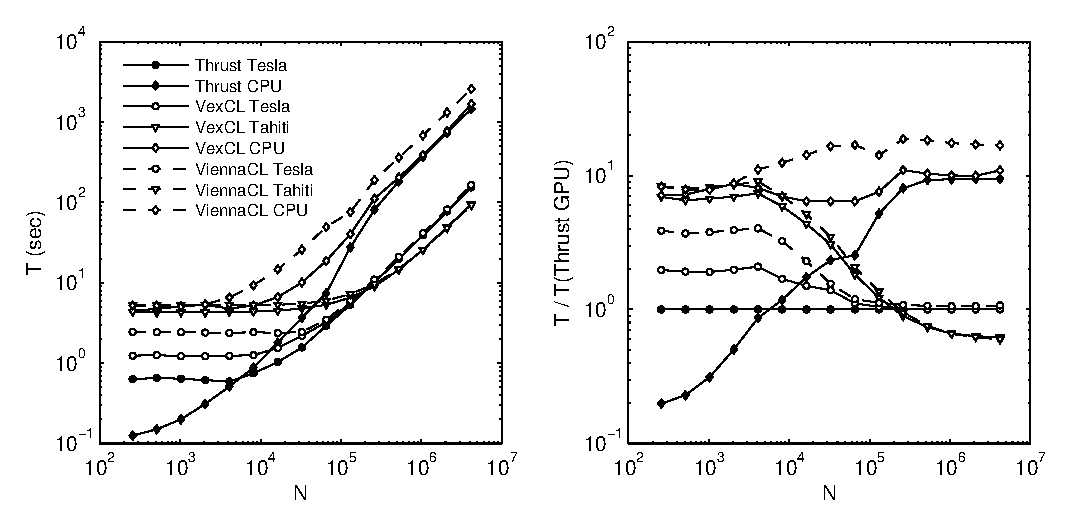
\includegraphics[width=\textwidth]{data/damped_oscillator/perfcmp}
    \end{center}
    \caption{Damped oscillator ensemble results}
    \label{fig:damped:perf}
\end{figure}

\begin{figure}[p]
    \begin{center}
        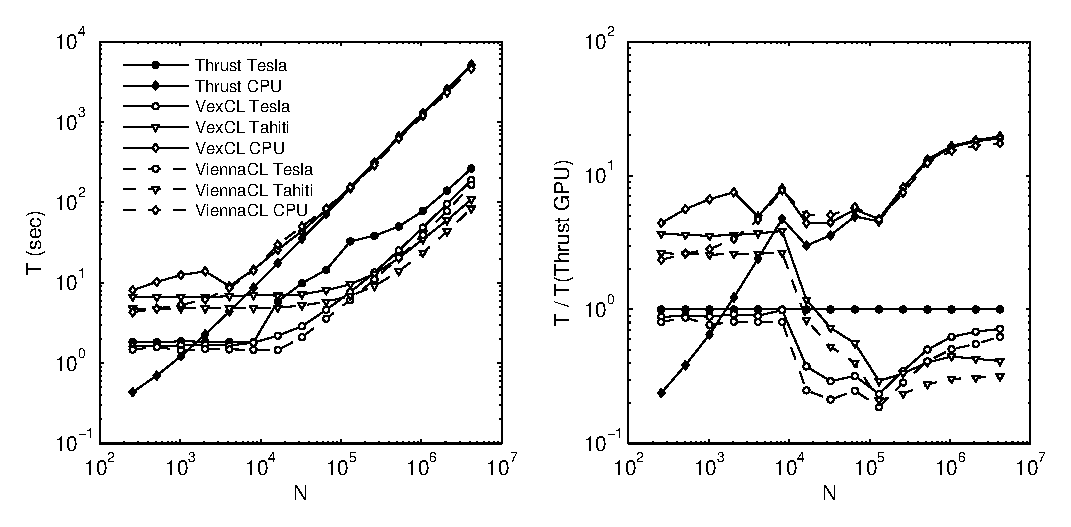
\includegraphics[width=\textwidth]{data/phase_oscillator_chain/perfcmp}
    \end{center}
    \caption{Coupled phase oscillator chain results}
    \label{fig:phase:perf}
\end{figure}

\begin{figure}[p]
    \begin{center}
        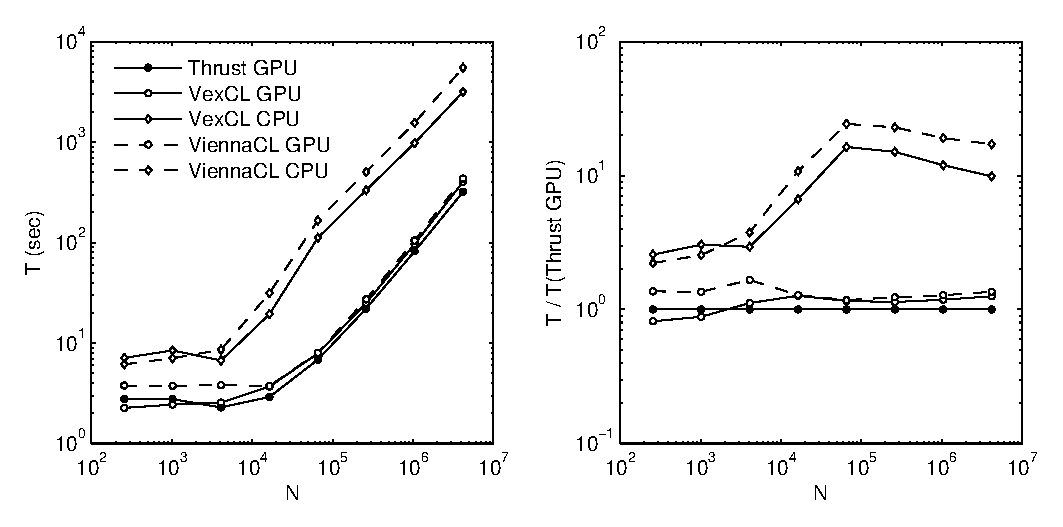
\includegraphics[width=\textwidth]{data/disordered_ham_lattice/perfcmp}
    \end{center}
    \caption{Disordered Hamiltonian lattice results}
    \label{fig:lattice:perf}
\end{figure}

\begin{figure}[p]
    \begin{center}
        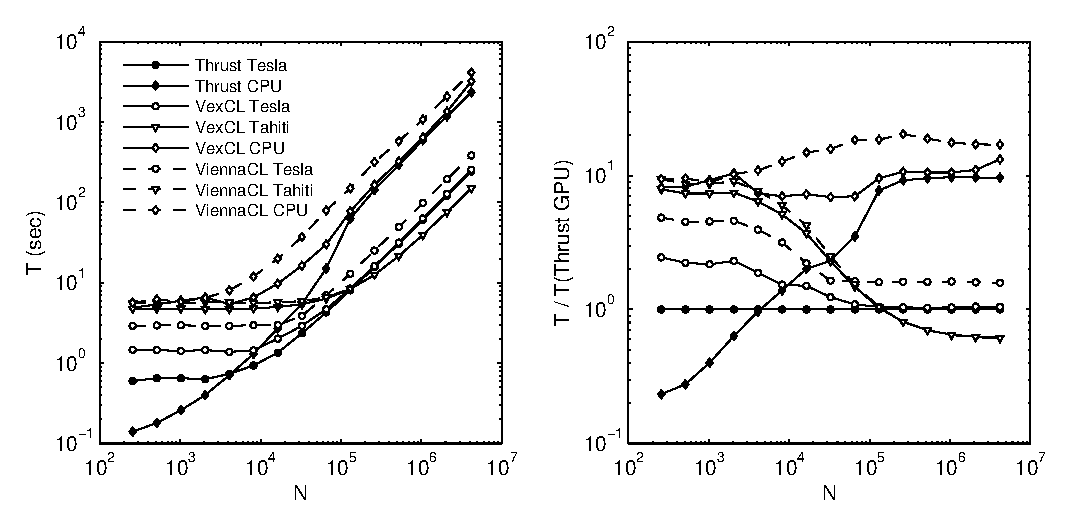
\includegraphics[width=\textwidth]{data/lorenz_ensemble/perfcmp}
    \end{center}
    \caption{Lorenz attractor ensemble results}
    \label{fig:lorenz:perf}
\end{figure}

\begin{figure}[p]
    \begin{center}
        \subfigure[
        Damped oscillator ensemble
	]{\label{fig:scaling:damped}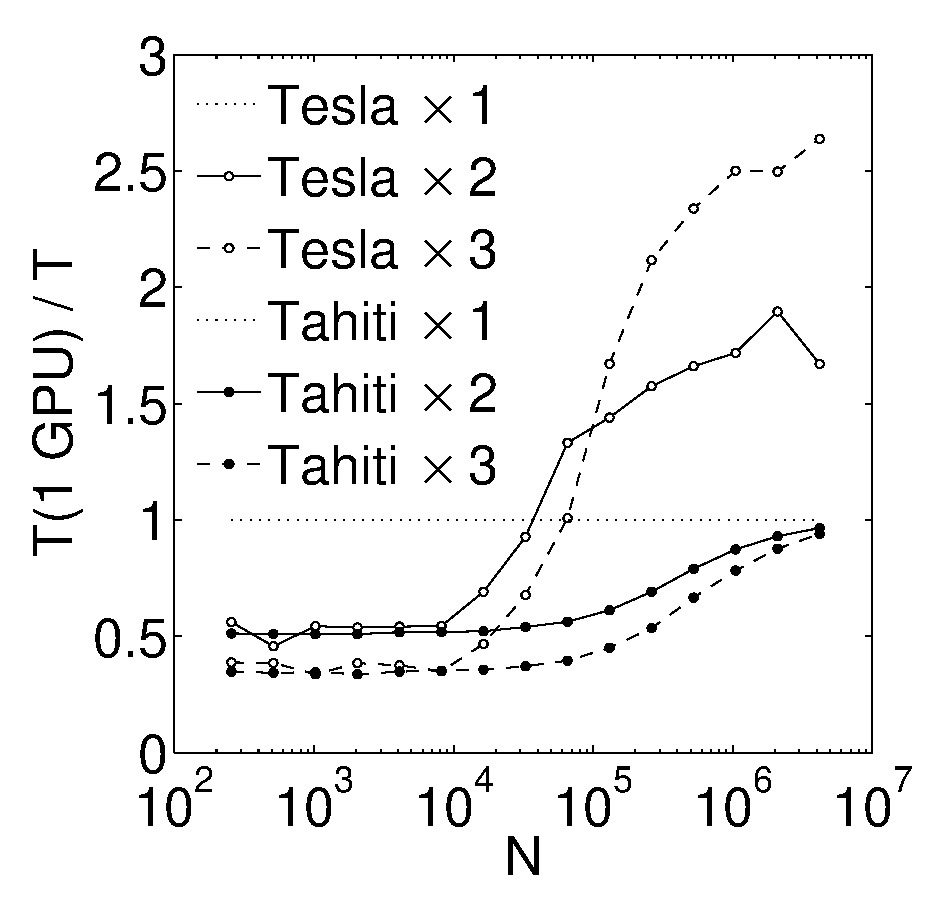
\includegraphics[width=0.45\textwidth]{data/damped_oscillator/scaling}}\quad
        \subfigure[
        Coupled phase oscillator chain
        ]{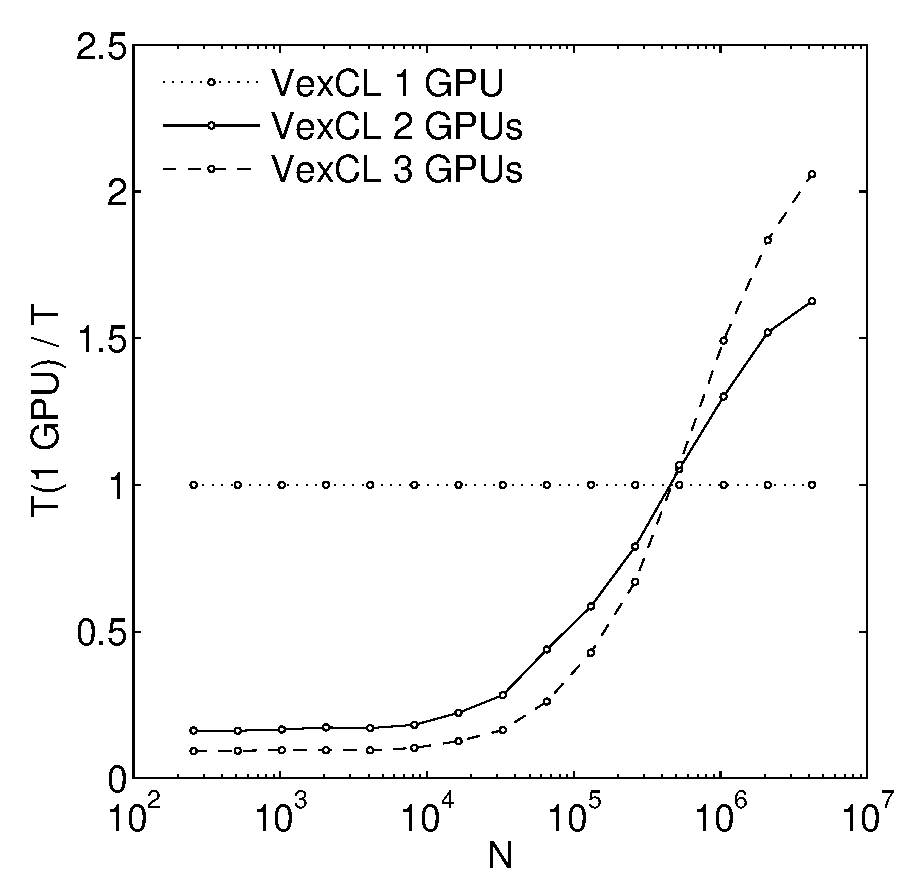
\includegraphics[width=0.45\textwidth]{data/phase_oscillator_chain/scaling}}\\
        \subfigure[
        Disordered Hamiltonian lattice
        ]{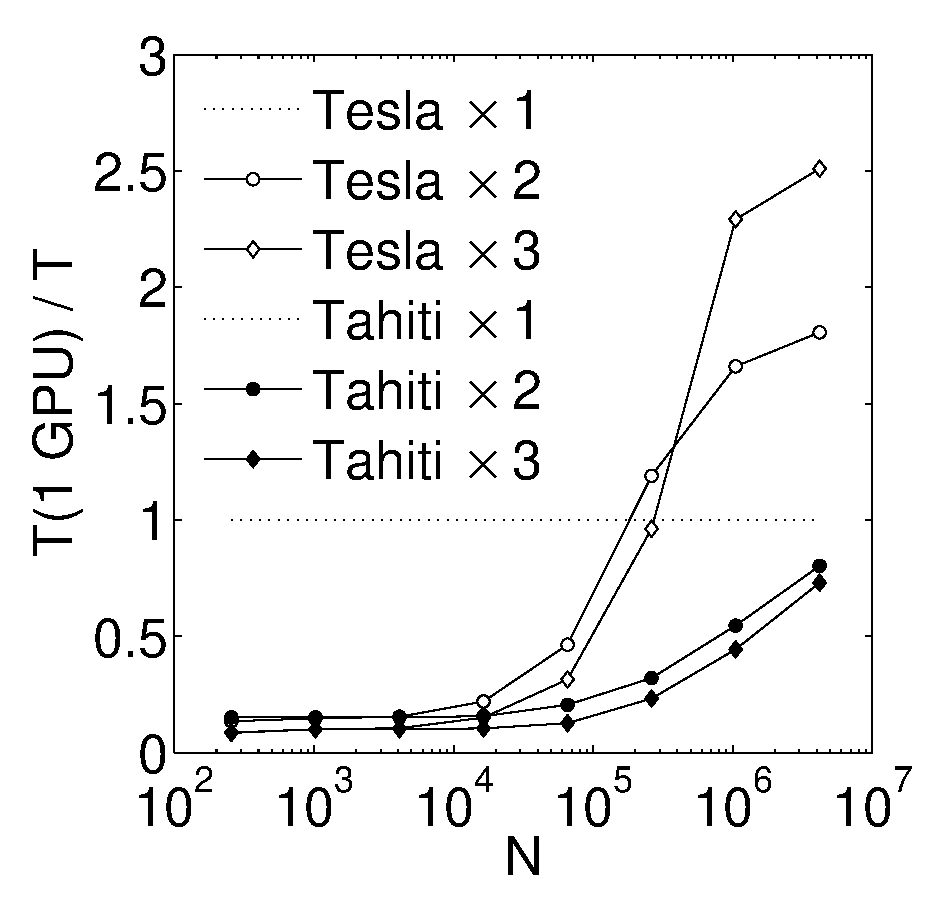
\includegraphics[width=0.45\textwidth]{data/disordered_ham_lattice/scaling}}\quad
        \subfigure[
        Lorenz attractor ensemble
        ]{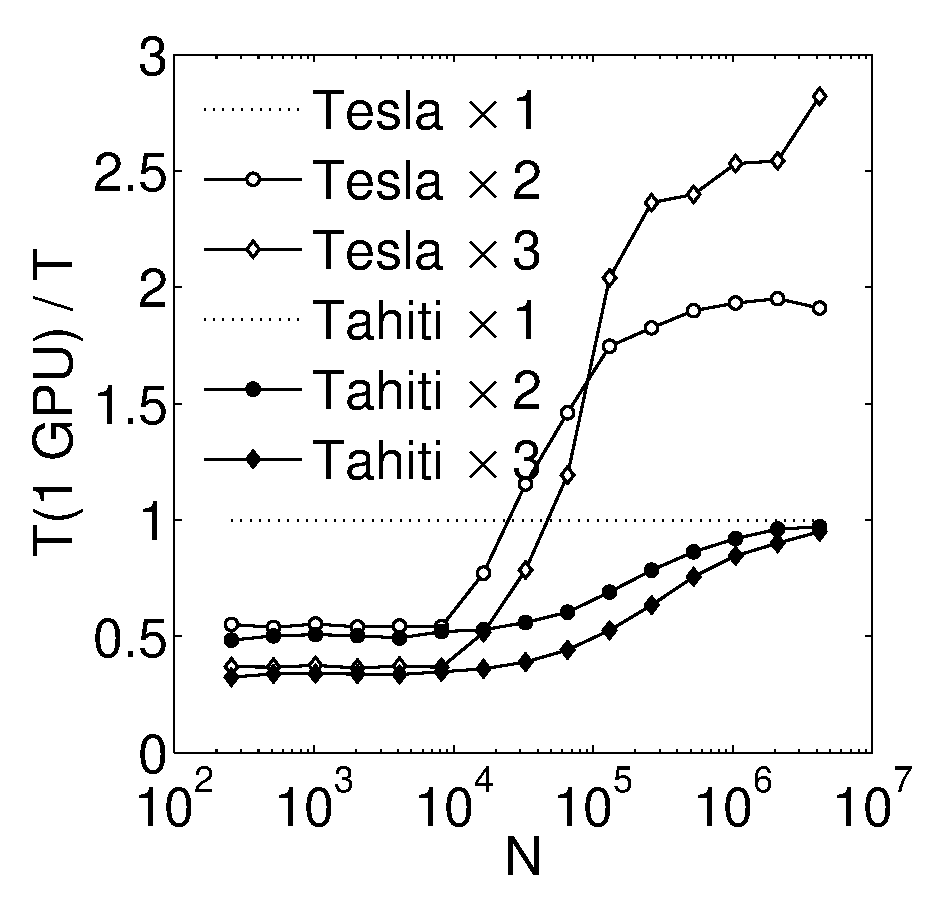
\includegraphics[width=0.45\textwidth]{data/lorenz_ensemble/scaling}}
    \end{center}
    \caption{VexCL scaling with multigpu computation}
    \label{fig:scaling}
\end{figure}









% 
% CONCLUSION
%
\section{Conclusion}

Performance-wise, there is almost no difference between various platforms and
libraries when those are run on the same hardware. As we have shown, various
computational problems may be solved effectively in terms of both human and
machine time with the help of modern high-level libraries.  There are some
differences in the programming interfaces of the libraries which may be crucial
for ones specific application. 

Thrust is more low-level and its interface is very close to the C++ STL
library.  The OpenCL libraries we looked at demonstrated that they are able to
provide more convenient interface for a scientific programmer than a direct
implementation in CUDA or OpenCL.  VexCL has richer set of elementwise vector
operations, while ViennaCL has extensive set of sparse linear systems solvers,
which we did not discuss in this paper.

Regarding a comparison of CUDA versus OpenCL, we believe that OpenCL has a
major difference with respect to CUDA. Namely, it has a  much wider range of
supported hardware, which is only going to extend with time because it is an
open standard supported by major hardware producers. The other OpenCL advantage
that we did not explore in this paper is the ability to generate kernels
optimized for the problem at hand at runtime. We believe that this feature has
good potential, but we leave its in-depth discussion for the future work.  On
the other hand, this feature of OpenCL may be considered its drawback: runtime
kernel compilation adds certain overhead notable for smaller workloads as has
been shown in this paper. 





\section{Acknowledgments}

This work has been partially supported by RFBR grant No 12-07-0007. We also
would like to thank Gradient JSC\footnote{ \href{
http://www.gradient-geo.com/en }{ http://www.gradient-geo.com/en } } for the
kindly provided AMD hardware.


\bibliographystyle{model1-num-names}
\bibliography{ref}

\end{document}
% vim: set et
